\subsection{Определение цепи Маркова}

Вспомним задачу с домашних заданий:

Петя хочет пойти в кино с вероятностью ровно $\frac{1}{3}$, а у него есть только честная монета. Может ли он осуществить свой замысел?

Как вы знаете она обладает вот таким решением:

\begin{center}
   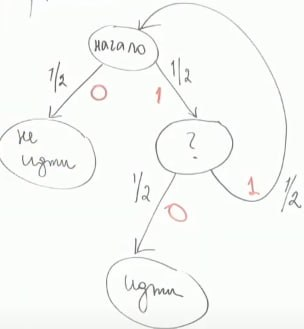
\includegraphics[width=8cm]{assets/5_1_1.jpg}
\end{center}

И действия Пети задаются этим орриентированным графом с весами на ребрах. Добавим петли в ребра идти и не идти с вероятностью 1.

Граф с конечным числом вершин, где на каждом ребре написаны вероятности, и где сумма чисел на ребрах исходящих из каждой вершины равна 1, называется \deff{цепь Маркова} или Марковская цепь. 

Посмотрим на распределение вероятностей. Посмотрим на вектор:

$b = (b_1,b_2,\ldots,b_n)$, где $b_i$ - вероятность оказаться в $i$ - ой позиции.

Возьмем матрицу $P$, где $p_{ij}$ - вероятность перейти из $i$ в $j$. Тогда на нашем примере была вот такая матрица:
$$P = \begin{pmatrix}
0&\frac{1}{2}&\frac{1}{2} & 0 \\
0& 1&0&0\\
\frac{1}{2}&0&0&\frac{1}{2}\\
0&0&0&1
\end{pmatrix}
$$
\deff{Поглощающее состояние} - то, которое переходит само в себя с вероятностью $1$.

Это \deff{матрица перехода} для цепи Маркова.

Пусть мы перешли в новое состояние: $c = (c_1,\ldots,c_n)$.
$$c_i = P(c = i) = \sum\limits_{j=1}^n P(c=i|B=j)P(b=j)=\sum\limits_{j=1}^n p_{ji}b_j$$
Откуда $c^T=b^TP$. Есть еще другое обозначение $\overrightarrow{c} = c^T$.

Посмотрим на наши шаги:

$b^0 = (1,0,0,0)$ - наш вектор $b$ изначально

$b^1 = (0,\frac{1}{2},\frac{1}{2},0)$

$b^2 = (\frac{1}{4},\frac{1}{2},0,\frac{1}{4})$

$b^3 = (0,\frac{5}{8},\frac{1}{8},\frac{1}{4})$

и так далее. Логично, что $\overrightarrow{b}^n = \overrightarrow{b} \cdot P^n$.

Мы смотрели с точки зрения линейной алгебры. Давайте посмотрим граф цепи Маркова (смотрим только ненулевые ребра). Тогда в нем есть такие виды вершин:
\begin{enumerate}
    \item поглощаюшие (существенное)
    \item непоглощающие (не существенное) - несколько выходов
\end{enumerate}

Цепь Маркова - \deff{поглощающая}, если из любого состояние можно дойти до поглощающего состояния.

\subsection{Эргодический класс}

\deff{Эргодический класс} - компонента сильной связности графа марковской цепи.

todo: вставить определение сильной связности.

Эргодический класс называется \deff{поглощающим}, если из него не исходит ребер в другие эргодические классы.

\deff{Конденсацией марковской цепи} называется конденсация графа.

\deff{Эргодическая марковаская цепь} - состоит из одного эргодического класса.

Эргодический класс \deff{периодическим} с периодом $d\neq 1$, если длина любого цикла в этом эргодическом классе делится на $d$ ($d$ - максимально).

\thmm{Теорема (о классификации марковских цепей)}

\begin{enumerate}
    \item $\forall$ марковская цепь содержит поглощающий эргодический класс.
    \item Марковская цепь с вероятностью $1$ рано или поздно оказывается в состоянии из поглощающего эргодического класса.
    \item для непереодического поглощающего эргодического класса в случае попадания в него существует стационнарное предельное распредельное вероятностей $b: b = bP$. $\forall$ начального распределение $b^0$, $b^0:b^0P^n\rightarrow b$.
\end{enumerate}

Жизнь Марковской цепи крайне скучна - А.С. Станкевич

\subsection{Уходим в математику.}

$b^1=b\cdot P$, $b^n = b \cdot P^n$

Дана поглащающая марковская цепь. Занумеруем, чтобы изначально шли непогл., а потом погл:

\begin{center}
   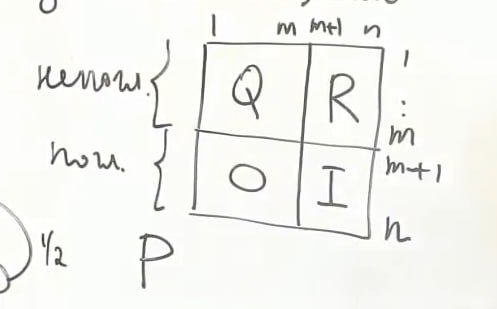
\includegraphics[width=8cm]{assets/5_3_1.jpg}
\end{center}

Где $I =$ единичная матрица.

Возьмем $a = $ началу вектора $b$, где любое состояние не поглощающее.

Заметим, что: $a^n = a \cdot Q^n$ из-за нулей. Докажем, что $Q^n \rightarrow 0$. 

\thmm{Теорема о поглощении.} 

Поглощающая М.Ц переходит в погл. состояние с вероятностью $1$.

todo: написать доказательство, оно несложное, я просто с температурой и не склеил

Хотим теперь понять, а где же мы поглотимся?

\subsection{Мат. ожидание времени до поглощения}

Давайте рассмотрим мат. ожидание времени до поглощения.

Есть $b_0$ - начальное распределение. $T$ - сл. величина: число шагов до погл:

$T=\sum\limits_{i=1}^m T_i$, где $T_i$ - число посещений $i$-ого состояния.

$T_i = \sum\limits_{j=0}^\infty = T_{ij}$, такая что $T_{ij} = \begin{cases}
    1, \text{ если на $j$-ом ходу в сост $i$}\\
    0, \text{ иначе}
\end{cases}$


$ET=\sum\limits_{i=1}^mET_i =\sum\limits_{i=1}^m\sum\limits_{j=0}^\infty E T_{ij} = \sum\limits_{i=1}^m(\sum\limits_{j=0}^\infty a^0Q^j)_i = \sum\limits_{i=1}^m(a_0\sum\limits_{j=0}^\infty Q^j)_i=\sum\limits_{i=1}^m(a_0N)_i$;

Как мы знаем из линейной алгебры: $\sum\limits_{j=0}^\infty Q^j = (I-Q)^{-1}$

$N = (I-Q)^{-1}$ - \deff{фундаментальная матрица} поглощающей марковской цепи.

$A = a^0NR$ - распределение вероятностей поглощения в состояниях




